\documentclass{beamer}
\beamertemplatenavigationsymbolsempty
\usepackage[french]{babel}
\usepackage{fontspec}
\usepackage{amsmath, amsthm, amsfonts}
\usepackage[separate-uncertainty]{siunitx}
\usepackage{xcolor}
\usepackage{tikz}
\usepackage{tikz-cd}
\usepackage[object=vectorian]{pgfornament}
\usepackage{circuitikz}
\usepackage{hyperref}
\usepackage{caption}
\usepackage{booktabs}
\usepackage{mathtools}
\usepackage{longtable}
\usepackage[version=3]{mhchem}
\usepackage{marginnote}
\usepackage[framemethod=tikz]{mdframed}


% Paul Tol's qualitative palette
% ``bright''.https://personal.sron.nl/~pault/#sec:qualitative
\definecolor{tblue}{HTML}{4477AA}
\definecolor{tcyan}{HTML}{66CCEE}
\definecolor{tgreen}{HTML}{228833}
\definecolor{tyellow}{HTML}{CCBB44}
\definecolor{tred}{HTML}{EE6677}
\definecolor{tpurple}{HTML}{AA3377}
\definecolor{tgrey}{HTML}{BBBBBB}


% Justification for marginnotes.
\renewcommand*{\raggedleftmarginnote}{}
\renewcommand*{\raggedrightmarginnote}{}


% Styles for mdframed environments.
\newmdenv[backgroundcolor=tgreen!10,linecolor=tgreen!30]{reponsebox}
\newmdenv[backgroundcolor=tyellow!10,linecolor=tyellow!30]{diapobox}
\newmdenv[backgroundcolor=tred!10,linecolor=tred!30]{fondamentalbox}

% Default arrow for tikz and style for positive and negative objects.
\tikzset{>=latex,
    negative/.style={draw=teal!70!black, fill=teal!10, thick},
    positive/.style={draw=red, fill=red!10, thick}}
\usetikzlibrary{matrix,calc,decorations.pathreplacing,decorations.pathmorphing,decorations.markings}

% French locale for numbers and negative exponent for units.
\sisetup{locale=FR, per-mode=symbol}

\newcommand{\abs}[1]{\left| #1 \right|}
\newcommand{\rhat}{\vec{\hat{r}}}
\newcommand{\xhat}{\vec{\imath}}
\newcommand{\yhat}{\vec{\jmath}}
\newcommand{\zhat}{\vec{k}}
\newcommand{\real}{\mathbb{R}}
\newcommand{\der}[2]{\frac{\mathrm{d}#1}{\mathrm{d}#2}}
\newcommand{\pder}[2]{\frac{\partial\ #1}{\partial\ #2}}
\newcommand{\dif}{\mathrm{d}}
\newcommand{\ddif}{\,\mathrm{d}}
\newcommand{\grad}{\vec{\nabla}}
\newcommand{\exemple}[1]{\begin{fullwidth}#1\end{fullwidth}}
\newcommand{\norm}[1]{\lVert\ #1\ \rVert}
\newcommand{\vu}{\vec{u}}
\newcommand{\vv}{\vec{v}}
\newcommand{\vr}{\vec{r}}
\newcommand{\va}{\vec{a}}
\newcommand{\vF}{\vec{F}}
\newcommand{\vE}{\vec{E}}
\newcommand{\vB}{\vec{B}}
\newcommand{\vecxyz}[3]{#1 \xhat\ + #2 \yhat\ + #3 \zhat}
\newcommand{\vecxy}[2]{#1 \xhat\ + #2 \yhat}
\newcommand{\coulombcst}{k}
\newcommand{\emf}{\ensuremath{\mathcal{E}}}
\newcommand{\eval}{\SI{1.602e-19}{C}}
\newcommand{\kval}{\SI{8.99e9}{Nm^2 \per C^2}}

% Nice separator line
\newcommand{\sectionline}{
    \noindent
    \begin{center}
        \resizebox{0.5\linewidth}{1ex}
    {{%
    {\begin{tikzpicture}
    \node  (C) at (0,0) {};
    \node (D) at (9,0) {};
    \path (C) to [ornament=85] (D);
    \end{tikzpicture}}}}
    \end{center}
}

\theoremstyle{definition}
\newtheorem*{defn}{Definition}


\usepackage[version=3]{mhchem}

\setbeamercolor{title}{fg=tblue}
\setbeamercolor{frametitle}{fg=tblue}
\setbeamercolor{structure}{fg=tblue}

% Make footnotesize smaller
\makeatletter
\renewcommand\footnotesize{%
   \@setfontsize\footnotesize\@viipt{11}%
   \abovedisplayskip 8\p@ \@plus2\p@ \@minus4\p@
   \abovedisplayshortskip \z@ \@plus\p@
   \belowdisplayshortskip 4\p@ \@plus2\p@ \@minus2\p@
   \def\@listi{\leftmargin\leftmargini
               \topsep 4\p@ \@plus2\p@ \@minus2\p@
               \parsep 2\p@ \@plus\p@ \@minus\p@
               \itemsep \parsep}%
   \belowdisplayskip \abovedisplayskip
}
\makeatother

\title{Électricité et magnétisme}
\subtitle{Chapitre 7 - Circuits en courant continu}
\date{26 octobre 2021}
\author{Loïc Séguin-Charbonneau}
\institute{Cégep Édouard-Montpetit}

\begin{document}

\maketitle

\begin{frame}[t]{Exercice sur la loi des n\oe uds}
  Le diagramme ci-dessous illustre un n\oe ud dans un circuit. Les courants sont
  \begin{align*}
    I_1 &= \SI{100}{mA} \\
    I_2 &= \SI{45}{mA} \\
    I_3 &= \SI{80}{mA} \\
    I_4 &= \SI{300}{mA} \\
  \end{align*}
  Déterminer $I_5$ et la direction du courant dans cette branche.

  \begin{center}
    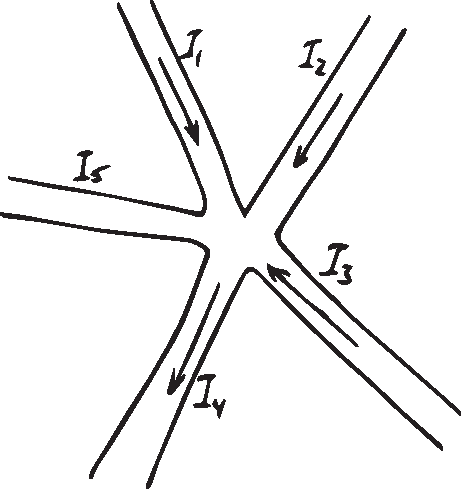
\includegraphics[scale=0.5]{figures/loi-noeuds.pdf}
  \end{center}
\end{frame}

\begin{frame}[t]{Exercice sur la loi des mailles}
  On considère le circuit suivant dans lequel $\emf = \SI{12}{V}$, $R_1 =
  \SI{100}{\ohm}$ et $R_3 = \SI{50}{\ohm}$. Le courant qui circule dans le
  circuit est de $I = \SI{30}{mA}$. Déterminer $R_2$.

  \begin{center}
  \begin{circuitikz}
    % French babel breaks everything... see https://latex.org/forum/viewtopic.php?t=11981
    \shorthandoff{:}\shorthandoff{!}
    \draw (0, 0)
      to[battery, l=\emf, invert] (0, 3)
      to[R, l=$R_1$] (4, 3)
      to[R, l=$R_2$] (4, 0)
      to[R, l=$R_3$] (0, 0);
  \end{circuitikz}
  \end{center}
\end{frame}


\begin{frame}{Pikachus en série et parallèle}
  Soit $R_{s}$ la résistance équivalente à trois Pikachus en série et $R_p$ la
  résistance équivalente à trois Pikachus en parallèle. On suppose que tous les
  Pikachus ont la même résistance.

  \begin{columns}
    \begin{column}{0.45\textwidth}
      \begin{center}
        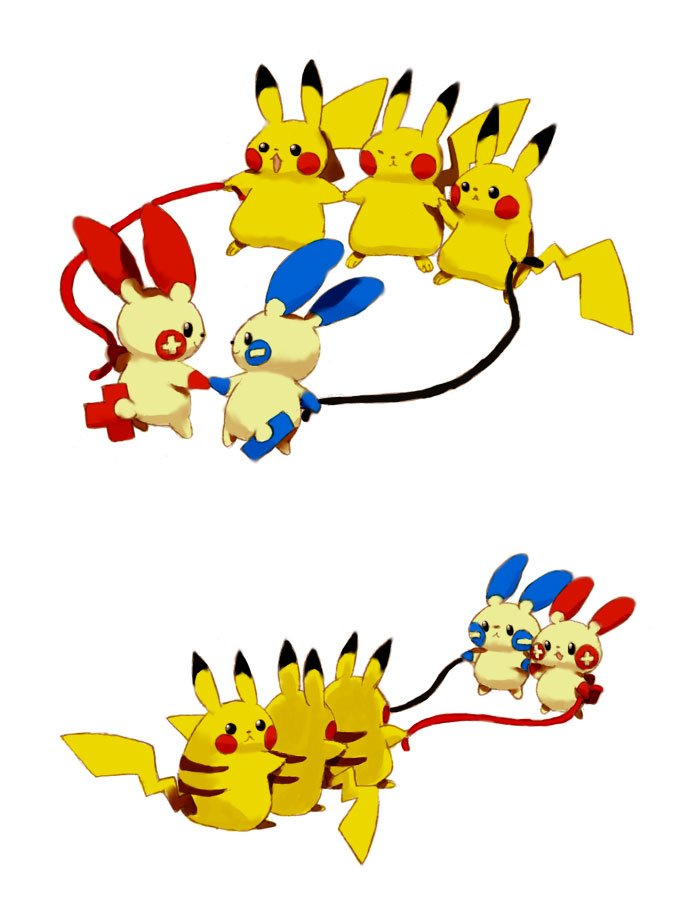
\includegraphics[width=4.5cm]{figures/series-parallel-pikachu.jpg}
      \end{center}
      \begin{flushright}
        {\tiny \url{http://i.imgur.com/4fPjx.jpg} }
      \end{flushright}
    \end{column}

    \begin{column}{0.55\textwidth}
      Quelle est la valeur du rapport $\frac{R_s}{R_p}$?

      \begin{enumerate}[A.]
        \item 9
        \item 3
        \item 1
        \item 1/3
        \item 1/9
      \end{enumerate}
    \end{column}
  \end{columns}
\end{frame}


\begin{frame}{Exemple de circuit à plusieurs mailles}
  \alt<1> {Trouvons le courant dans chaque branche}{}
  \alt<2> {{\color{black!50!green} Identifier la direction du courant (au hasard!)}}{}
  \alt<3> {{\color{black!40!red} Identifier la direction des mailles et le n\oe ud}}{}

  \begin{center}
    \begin{circuitikz}
      % French babel breaks everything... see https://latex.org/forum/viewtopic.php?t=11981
      \shorthandoff{:}\shorthandoff{!}
      \draw (0, 0) to[R=$R_1$] (0, 4)
        to[battery, l=$\emf_1$] (4, 4);
      \draw (4, 4) to[R=$R_3$] (8, 4)
        to (8, 0)
        to[R=$R_4$] (4, 0)
        to (0, 0);
      \draw (4, 0) to[battery, l=$\emf_2$] (4, 2)
        to[R=$R_2$] (4, 4);
      \only<2> {
        \draw[->, black!50!green, ultra thick] (2.5, 0.3) -- node[above] {$i_1$} ++(-1, 0);
        \draw[<-, black!50!green, ultra thick] (4.5, 2.5) -- node[right] {$i_2$} ++(0, -1);
        \draw[->, black!50!green, ultra thick] (5.5, 3.6) -- node[below] {$i_3$} ++(1, 0);
      }
      \only<3-> {
        \draw[->, black!50!green, thick] (2.5, 0.3) -- node[above] {$i_1$} ++(-1, 0);
        \draw[<-, black!50!green, thick] (4.5, 2.5) -- node[right] {$i_2$} ++(0, -1);
        \draw[->, black!50!green, thick] (5.5, 3.6) -- node[below] {$i_3$} ++(1, 0);
      }
      \only<3> {
        \draw[black!40!red, ultra thick, ->] (2, 2) node {$1$} ++(230:0.6) arc(230:-50:0.6);
        \draw[black!40!red, ultra thick, ->] (6, 2) node {$2$} ++(230:0.6) arc(230:-50:0.6);
        \fill[black!40!red] (4, 4) circle (3pt);
        \node[above] at (4, 4) {\color{black!40!red} $a$};
      }
      \only<4-> {
        \draw[black!40!red, thick, ->] (2, 2) node {$1$} ++(230:0.6) arc(230:-50:0.6);
        \draw[black!40!red, thick, ->] (6, 2) node {$2$} ++(230:0.6) arc(230:-50:0.6);
        \fill (4, 4) circle (1.5pt);
        \node[above] at (4, 4) {$a$};
      }
    \end{circuitikz}
  \end{center}
\end{frame}


\begin{frame}{Batterie d'ordinateur}
  Un ordinateur portable a une batterie de \SI{49.9}{\watt\hour} avec une
  f.é.m. de \SI{11.4}{\volt}. L'ordinateur vient avec un chargeur de
  \SI{30}{\watt}. Lorsque la batterie fournit un courant de
  \SI{800}{\milli\ampere} à l'ordinateur, la différence de potentiel à ses
  bornes chute à \SI{10.9}{\volt}. 

  \begin{enumerate}
    \item Quelle est la résistance interne de la batterie?
    \item Quelle est la puissance perdue sous forme de chaleur dans la batterie?
    \item Si la batterie est complètement vide au départ, combien de temps est
      nécessaire pour la charger complètement? (Vous pouvez négliger la
      résistance interne ici.)
  \end{enumerate}

\end{frame}


\begin{frame}{Défibrillateur cardiaque}
  \begin{center}
    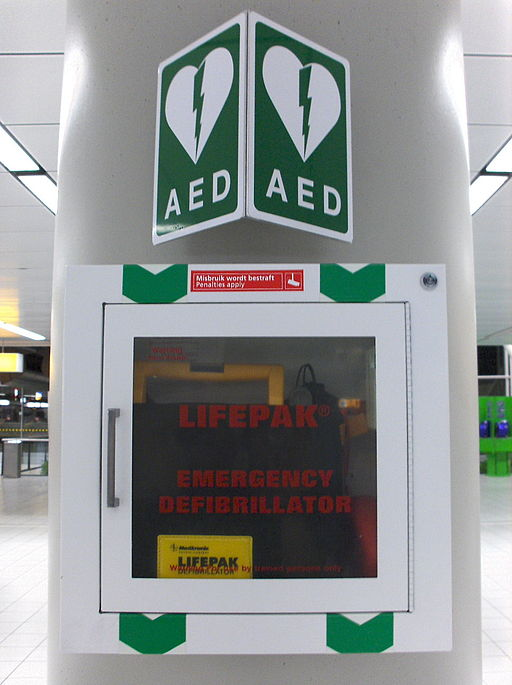
\includegraphics{figures/Defibrillator.jpg}
  \end{center}
\end{frame}


\begin{frame}{Défibrillateur}
Un défibrillateur cardiaque est composé d'une source de tension dont la fém est
\SI{2500}{V} et d'un condensateur de \SI{32}{\micro\farad}. Pour charger le
condensateur, on le place en série avec une résistance de \SI{10}{\kilo\ohm}.

Quel est le temps requis pour que le condensateur atteigne \SI{95}{\percent} de
sa charge maximale?

\end{frame}


\begin{frame}{Défibrillateur}

Maintenant que le condensateur est chargé, on peut utiliser le défibrillateur.
On connecte le condensateur en série avec le c\oe ur et le condensateur se
décharge à travers ce dernier. La décharge dans le c\oe ur prend \SI{5}{ms} et
est complète lorsqu'il ne reste que \SI{10}{\percent} des charges initiales
sur le condensateur. Quelle est la résistance du thorax?

Quel était le courant dans le c\oe ur \SI{1}{ms} après le
début de la décharge?

Quelle est l'énergie qui est fournie par le condensateur au c\oe ur?
\end{frame}


\end{document}
